% Created 2021-04-02 Fri 13:43
% Intended LaTeX compiler: pdflatex
\documentclass[english,zadani,odsaz]{fitthesis}
\renewcommand\title[1]{}
\usepackage{minted}
\usepackage{tikz}
\usepackage{tikz-cd}
\usepackage{bussproofs}
\usepackage[figure,table,listing]{totalcount}
\projectinfo{
  project={DP},
  year={2021},
  date=\today,
  title.cs={Just-in-time překlad závisle typovaného lambda kalkulu},
  title.en={Just-in-Time Compilation\\of the Dependently-Typed Lambda Calculus},
  title.length={15.5cm},
  %sectitle.length={14.5cm}, % nastavení délky bloku s druhým titulkem pro úpravu zalomení řádku (lze definovat zde nebo níže)
  author.name={Jakub},
  author.surname={Zárybnický},
  author.title.p={Bc.},
  department={UITS},
  supervisor.name={Ondřej},
  supervisor.surname={Lengál},
  supervisor.title.p={Ing.},
  supervisor.title.a={Ph.D.},
  faculty={FIT},
  faculty.cs={Fakulta informačních technologií},
  faculty.en={Faculty of Information Technology},
  department.cs={Ústav inteligentních systémů},
  department.en={Department of Intelligent Systems},
  keywords.cs={Truffle, Virtuální stroj JVM, just-in-time překlad, tvorba překladačů, závislé typy, lambda kalkul},
  keywords.en={Truffle, Java Virtual Machine, just-in-time compilation, compiler construction, dependent types, lambda calculus},
  abstract.en={
   A number of programming languages have managed to greatly improve their
   performance by replacing their custom runtime system with general platforms
   that use just-in-time optimizing compilers like GraalVM or RPython. This
   thesis evaluates whether such a transition would also benefit
   dependently-typed programming languages or theorem provers.

   This thesis introduces the type-theoretic notion of dependent types and the
   algorithms involved in working with them, specifies a minimal
   dependently-typed language on the $\lambda\Pi\text{-calculus}$, and presents
   the implementation two interpreters for this language: a simple interpreter
   written in Kotlin, and a second interpreter, also written in Kotlin, that
   uses the Truffle language implementation framework on the GraalVM platform,
   which is a partial evaluation-based just-in-time compiler based on the Java
   Virtual Machine. The performance of these two interpreters is then compared
   on a number of normalization and elaboration tasks.

   [...specific numbers]
  }, abstract.cs={

   Řada programovacích jazyků byla schopna zvýšit svoji rychlost nahrazením
   běhových systémů, stavěných pouze pro potřeby jazyka, obecnými platformami,
   které pro optimalizaci používají just-in-time překlad, jako jsou GraalVM nebo
   RPython. Tato práce vyhodnocuje, zda je použití takovýchto platforem vhodné i
   pro jazyky se závislymi typy nebo důkazovými systémy.

   Tato práce představuje koncepty $\lambda\text{-kalkulu}$ a teorie typů
   potřebné pro úvod do závislých typů a algoritmy, které jsou potřeba pro práci
   s nimi, specifikuje malý závisle-typovaný jazyk založený na
   $\lambda\Pi\text{-kalkulu}$, a prezentuje dva interpretery tohoto jazyka:
   jednoduchý interpreter ve funkcionálním stylu psaný v jazyce Kotlin, a druhý
   interpreter, taktéž psaný v jazyce Kotlin, který používá platformu GraalVM a
   Truffle, knihovnu pro vytváření programovacích jazyků. GraalVM je platforma
   založená na virtuálním stroji Javy (JVM), která přidává just-in-time
   překladač založený na částečném vyhodnocení (\textit{partial evaluation}). Na
   závěr práce vyhodnocuje běhové charakteristiky těchto interpreterů na různých
   zátěžových testech.

   [...vyhodnocení]
  },
  extendedabstract={
  Systémy, které používají závislé typy, umožňují programátorům vytvářet
  programy, které jsou zaručeně správné vzhledem k vlastnostem, které mají
  uložené v typech. Tyto systémy je také možné použít pro logické nebo
  matematické důkazy, nebo pro dokazování správnosti celých systémů.  Poslední
  roky přinesly mnoho pokroků v teorii typů, na níž jsou tyto systémy založené,
  jako např. kvantitativní nebo homotopické typy. Vysoké nároky na důkazové schopnosti
  systémů s sebou ale prináší problémy s výkonem, konkrétně rychlostí kontroly
  typů (\textit{type-checking}, \textit{elaboration}). V této práci zhodnocuji
  vhodnost just-in-time překladu pro takové systémy, což je jeden z obecných
  přístupů pro optimalizaci rychlosti systémů.

  V první části vysvětluji principy typovaného $\lambda\text{-kalkulu}$, na němž
  jsou systémy se závislými typy založené, základy teorie typů a konkrétní
  specifikace několika rozšíření, které poté používám pro specifikaci malého
  jazyka.

  V druhé sekci pokračuji představením algoritmů, které jsou potřeba pro práci
  se závislými typy: \textit{normalization-by-evaluation} a
  \textit{bidirectional typing}. Tyto implementuji a používám pro vytvoření
  funkčního interpreteru tohoto jazyka.

  Třetí sekce představuje detaily platformy GraalVM a knihovny Truffle, které
  poté používám pro implementaci druhého interpreteru, který využívá
  just-in-time překladu.

  V závěru práce vyhodnocuji [...]

  Vyhodnocení, přínos práce
  },
  declaration={
    I hereby declare that this Master's thesis was created as an original work
    by the author under the supervision of Ing. Ondřej Lengál Ph.D.

    I have listed all the literary sources, publications, and other sources
    that were used during the preparation of this thesis.
  },
  acknowledgment={
    I would like to thank my supervisor Ing. Ondřej Lengál Ph.D. for entertaining a
    second one of my crazy thesis proposals.

    I would like to thank Edward Kmett for suggesting this idea: it has been a
    challenge.

    I would also like to thank my family and friends who supported me when I needed
    it the most throughout my studies.
  }
}

\date{\today}
\title{}
\hypersetup{
 pdfauthor={},
 pdftitle={},
 pdfkeywords={},
 pdfsubject={},
 pdfcreator={Emacs 28.0.50 (Org mode 9.3)}, 
 pdflang={English}}
\begin{document}

% * (front matter)                                              :ignoreheading:
\maketitle
\setlength{\parskip}{0pt}
{\hypersetup{hidelinks}\tableofcontents}
\iftotalfigures\listoffigures\fi
\iftotaltables\listoftables\fi
\iftotallistings\listoflistings\fi
\iftwoside\cleardoublepage\fi
\setlength{\parskip}{0.5\bigskipamount}

\chapter{Změnit název: ``Montuno: Efficient elaboration of dependent types using JIT compiler''}
\label{sec:org605e2a9}

\chapter{Introduction}
\label{sec:org44f3e9a}
\section{(Old)}
\label{sec:org2ef14f0}
When creating small experimental or research languages, writing a compiler may
be too much effort for the expected gain. On the other hand an interpreter is
usually not as performant as its creators may require for more computationally
intensive tasks.

There is a potential third way, proposed by Yoshihiko Futamura in the 1970s,
called the Futamura projection (or partial program evaluation), wherein an
interpreter is specialized in conjunction with the source code of a program,
yielding an executable. Some parts of the interpreter may be specialized, some
optimized, some left off entirely. Depending on the quality of the specializer,
the gains may be several orders of magnitude.

The goal of my thesis is to evaluate whether the GraalVM/Truffle platform is
suitable enough to act as a specializer for functional languages, in particular
for the dependently-typed lambda calculus.  To illustrate in Figure
\ref{fig:futamora}, the question is whether the path \textit\{Native
Image\textrightarrow Result\} is fast enough compared to the path
\textit{Executable\textrightarrow Result}.

\begin{figure}
\centering
\begin{tikzcd}
{} & Program
 \arrow[ld, "Compiler" description, bend right]
 \arrow[dd, "Interpreter" description, bend right=67]
 \arrow[rd, "Partial\ Evaluation" description, bend left]
 \arrow[dd, "JIT" description, bend left=67] & {} \\
Executable \arrow[rd, "Run" description, bend right] & {} & Native\ Image \arrow[ld, "Run", bend left]
 \\ {} & Result & {}
\end{tikzcd}
\caption{Methods of program execution}
\label{fig:futamora}
\end{figure}

Truffle has already been used rather successfully for the (mostly) imperative
languages Ruby, Python, R, Java, and WebAssembly, but (purely-)functional
languages differ in their evaluation model and in particular the required
allocation throughput, so it is still an open question whether GraalVM is a good
enough fit.

The desired outcome---at least, of the first part of my thesis---is a set of
implementations, and a set of benchmarks demonstrating a positive or a negative
result.  If the result is positive, there are many potential follow-up tasks:
implementing a different, more complex language, maybe a language to be
interpreted into the dependently-typed lambda calculus to attempt the approach
implemented in the \emph{Collapsing Tower of Interpreters} \cite{amin2017collapsing},
or experimenting with different runtime models - all depending on the results of
this preliminary proof of concept.

In the best case, the JIT-compiled program would be as close in performance to a
program processed by a hand-crafted compiler as possible (not including JIT
warm-up), and I would spend the second half of my thesis on different topics
(like provably-correct program transformations) instead of hand-optimizing the
primitive operations - I should find out which it is going to be as soon in the
second term as possible.

As far as I am aware, there are no other native just-in-time compiled
implementations of the dependently-typed lambda calculus, with the exception of
the preliminary investigations done by the originator of this idea
\cite{kmett_2019}, although there are a few projects implementing a lambda
calculus directly to the Java Virtual Machine byte code..

\section{New}
\label{sec:org87d7d5a}
--- see Excel@FIT start

Follow-up to Cadenza (STLC) on behalf of its creator

Combination of JIT and dependent types is natural (computation on the type-level) but not found in literature

Motivation: JIT for elaboration!!! plus easy prototyping, stepping block for
    other projects (efficient LF/Twelf, \ldots{})

smalltt a step in another direction


\chapter{GraalVM and the Truffle Framework}
\label{sec:org55e978c}
\section{Intro: ecosystem, purpose, benefits}
\label{sec:orgb9a70cc}
\textbf{GraalVM} is a just-in-time optimizing compiler for the Java bytecode. \textbf{Truffle} is
a set of libraries that expose the internals of the GraalVM compiler, intended
for easy implementation of other languages. So far JavaScript, Python, Ruby, R,
and WebAssembly have Truffle implementations, and therefore can run on the JVM.

GraalVM is also intended to allow creating \emph{polyglot applications} easily,
applications that have their parts written in different languages. It is
therefore easy to e.g. call R to create visualizations for the results of a
Python program, or to call any Truffle language from Java.

There is also the option to compile a \emph{Native Image} to eliminate most program
start-up costs associated with a just-in-time compiler, pre-compiling the
program partially (ahead-of-time).

From the point of view of a programmer, Truffle makes it possible to write an
interpreter, and then slowly add optimizations like program graph rewriting,
node specializations, inline instruction caching or others. This seems like a
good middle ground between spending large amounts of time on an optimized
compiler, and just specifying the semantics of a program in an interpreter that,
however, will likely not run quickly.

While GraalVM/Truffle is open-source and released under GPL v2, an
enterprise edition that claims large performance improvements is released
commercially.

\begin{figure}[!htb]
\centering
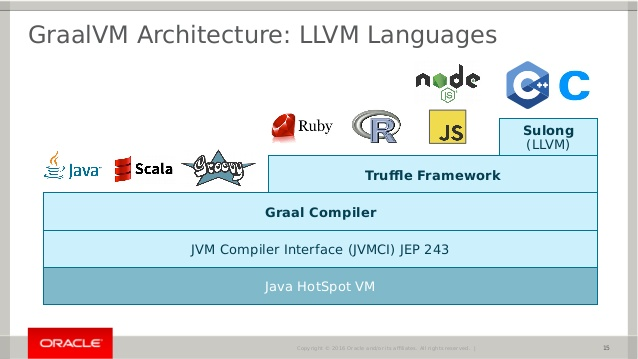
\includegraphics[width=.9\linewidth]{./img/graalvm.jpg}
\caption{GraalVM and Truffle (source: oracle.com)}
\end{figure}

JIT options - specialization, deoptimization
Use cases
Potential optimizations
\section{GraalVM}
\label{sec:orgcc19adc}
marketing texts

diagrams

Hotspot's JIT vs Graal's

\section{Truffle}
\label{sec:org9dbdbb8}
Intro + motivating multilanguage snippet

features with code samples

benchmarks for other languages

\chapter{Language specification}
\label{sec:orgc59e533}
\section{Dependent types}
\label{sec:org0762d55}
Intro dependent types + motivating example

hot ML research area (cubical, path, \ldots{}) (look in Kovacs' materials)

\section{Lambda Calculus Theory}
\label{sec:org8d4a078}
\subsection{Untyped Lambda Calculus}
\label{sec:orgbd1c553}
The untyped lambda calculus is a simple language consisting of just three kinds
of forms: variables, function application, and abstraction.

\begin{figure}[!htpb]
\[\begin{array}{ccll}
e & ::= & x            & \text{variable} \\
  & |   & e_1~e_2      & \text{application} \\
  & |   & \lambda x. e & \text{abstraction}
\end{array}\]
\caption{Untyped lambda calculus}
\end{figure}

syntax, semantics, usage

\subsection{Simply-Typed Lambda Calculus}
\label{sec:org16662a1}
The simply-typed lambda calculus adds a fourth kind of a term, type annotation,
and its type language:

\begin{figure}[!htpb]
\[\begin{array}{ccll}
e & ::= & x           & \text{variable} \\
  & |   & e_1~e_2      & \text{application} \\
  & |   & \lambda x. e & \text{abstraction} \\
  & |   & x:\tau     & \text{annotation}
\end{array}\]
\[\begin{array}{ccll}
\tau & ::= & \alpha           & \text{base type} \\
     & |   & \tau\rightarrow\tau' & \text{composite type}
\end{array}\]
\caption{Simply typed lambda calculus}
\end{figure}

syntax, semantics, type checking, type inference

\subsection{Dependently-Typed Lambda Calculus}
\label{sec:orgd3dc091}

Lambda cube

\ldots{} image

The dependently typed lambda calculus merges these two languages together,
simplifying the grammar.

\begin{figure}[!htpb]
\[\begin{array}{ccll}
e & ::= & x           & \text{variable} \\
  & |   & e_1~e_2      & \text{application} \\
  & |   & \lambda x. e & \text{abstraction} \\
  & |   & x:\tau      & \text{annotation} \\
  & |   & *           & \text{the type of types} \\
  & |   & \forall x:\rho.\rho' & \text{dependent function space}
\end{array}\]
\caption{Dependently typed lambda calculus}
\end{figure}
\ldots{}

directions, decidability, where is DTLC

implicits, holes, metacontext

\section{Algorithms}
\label{sec:org8c81d3d}
type-checking (bidi, NbE) + motivation

elaboration (what is it, why is it slow, glued, nondet, cite Kovacs)

evaluation techniques (by-need, \ldots{})

eval/apply (in implementation section)

\section{Specification}
\label{sec:org6d14800}
\begin{listing}[!htpb]
\begin{minted}[]{text}
let const = (\ a b x y -> x) :: forall (a :: *) (b :: *) . a -> b -> a
\end{minted}
\caption{The constant function in LambdaPi}
\end{listing}

grammar

semantics (inference rules, evaluation rules)

\chapter{Language Implementations}
\label{sec:orgdf575c8}
\section{Pure Interpreter}
\label{sec:org26ee3d5}
\subsection{Parser}
\label{sec:org7cfeb08}
ANTLR is the parser to use in JVM

Several ways to consume: listener, visitor - I've used AST transformation which
is the most compact and most familiar to other DTLC implementations which are
usually in functional languages

(listener - enter/exit function calls, visitor is similar, toAst uses recursive calls)

\begin{minted}[linenos,firstnumber=1]{antlr}
grammar Montuno;
@header {
package montuno;
}

file : (decls+=top)* EOF;

top
    : id=IDENT ':' type=term '.' #Decl
    | id=binder (':' type=term)? '=' body=term '.' #Defn
    | '%nf' term #Elab
    ;

term
    : 'let' name=binder ':' type=term '=' tm=term 'in' body=term #Let
    | LAMBDA (args+=binder)* '.' body=term #Lam
    | '(' (dom+=binder)+ ':' kind=term ')' ARROW cod=term #PiExpl
    | '{' (dom+=binder)+ (':' kind=term)? '}' ARROW cod=term #PiImpl
    | (spine+=atom)+ (ARROW rest=term)? #App
    ;
atom
    : '(' rec=term ')' #Rec
    | IDENT #Var
    | '*' #Star
    | 'Nat' #Nat
    | NAT #LitNat
    ;
binder
    : IDENT #Ident
    | '_' #Hole
    ;

IDENT : [a-zA-Z] [a-zA-Z0-9']*;
NAT : [0-9]+;

WS : [ \t\r\n] -> skip;
COMMENT : '--' (~[\r\n])* -> skip;
NCOMMENT : '{-'~[#] .*? '-}' -> skip;
LAMBDA : '\\' | 'λ';
ARROW : '->' | '→';
\end{minted}

\subsection{Data shape}
\label{sec:org1cf8b82}

\subsection{Algorithms}
\label{sec:orgc23ee08}
elaboration

\section{Truffle Interpreter}
\label{sec:orgd235983}
I have implemented a dependently typed lambda calculus called LambdaPi based on
the prior work \emph{A tutorial implementation of a dependently typed lambda calculus}
\cite{loh2010tutorial}. The parser and interpreter are written in Kotlin, where
I will also need to write the JIT implementation. This is a pure interpreter
that will serve as a baseline for future benchmarks.

parser shared with the previous implementation

data classes

truffle specifics

inline cache, tail call, trampoline (continuations)

!! show their effect on program graphs

eval/uneval(quote)

evaluation phases - translate to Code, run typecheck, run eval vs glued, ???

native image

\subsection{Evaluation model of function application}
\label{sec:org541f92d}
push-enter - arguments are pushed onto the stack, the function then takes as
many as it requires

eval-apply - the caller sees the arity of the function and then decides whether
it is over-applied (evaluates the function and creates a continuation), appllied
exactly (EVAL), or under-applied (creates a PAP, a closure-like value)

-- exactly describe the rules from eval-apply paper KNOWNCALL, EXACT, CALLK, PAP
-- known application ( = known arity), unknown function


\section{Similar implementations}
\label{sec:orgea74763}
``I've considered LLVM, WASM backends, but we need to evaluate type-checking
perf especially, so not relevant - better to compare with existing and/or
experimental systems''

SmallTT, Coq, Agda, GHC - for comparison

\chapter{Evaluation}
\label{sec:orgf507896}
\section{Benchmarks}
\label{sec:org8a6ee3e}
\begin{itemize}
\item from SmallTT project, from Idris project
\item memory usage (curve)
\item compilation speed (type-heavy test)
\item evaluation speed (compute-heavy test)
\end{itemize}

Nats, pairs, fun types, numerics

\section{Results}
\label{sec:orgea99192}
---

\section{Future work}
\label{sec:orgbec03ed}
good enough?

LF, techniques, extensions, real language

\chapter{Conclusion}
\label{sec:org7079550}




% * (bibliography, start of appendix)                           :ignoreheading:

\makeatletter
\def\@openbib@code{\addcontentsline{toc}{chapter}{Bibliography}}
\makeatother
\begin{flushleft}

\bibliographystyle{bibstyle}
\bibliography{bibliography}

\end{flushleft}
\iftwoside\cleardoublepage\fi
\appendix
\appendixpage
\iftwoside\cleardoublepage\fi
\startcontents[chapters]
% \setlength{\parskip}{0pt}
% \printcontents[chapters]{l}{0}{\setcounter{tocdepth}{2}}
% \setlength{\parskip}{0.5\bigskipamount}
\iftwoside\cleardoublepage\fi

\chapter{Contents of the attached data storage}
\label{sec:org19b42c7}
\ldots{}
\end{document}